\documentclass{article}

\usepackage{array}
\usepackage[margin=1in]{geometry}
\usepackage[utf8]{inputenc}
\usepackage[T1]{fontenc}
\usepackage{graphicx}
\usepackage{xcolor}
\usepackage{amssymb}
\usepackage{amsmath}
\usepackage{cancel}

\author{Uzair Akram}

\newcommand*\Eval[3]{\left.#1\right\rvert_{#2}^{#3}}
\newcommand\rd[1]{\textcolor{red}{\itshape #1}}
\newcommand\orn[1]{\textcolor{orange}{\itshape #1}}
\newcommand\blu[1]{\textcolor{blue}{\itshape #1}}

\pagenumbering{gobble}

\begin{document}
\section*{Fundamental Theorem of Calculus - A Proof by Definition}

\begin{tabular}{l l}
\textbf{Derivative}  \hspace{2cm} 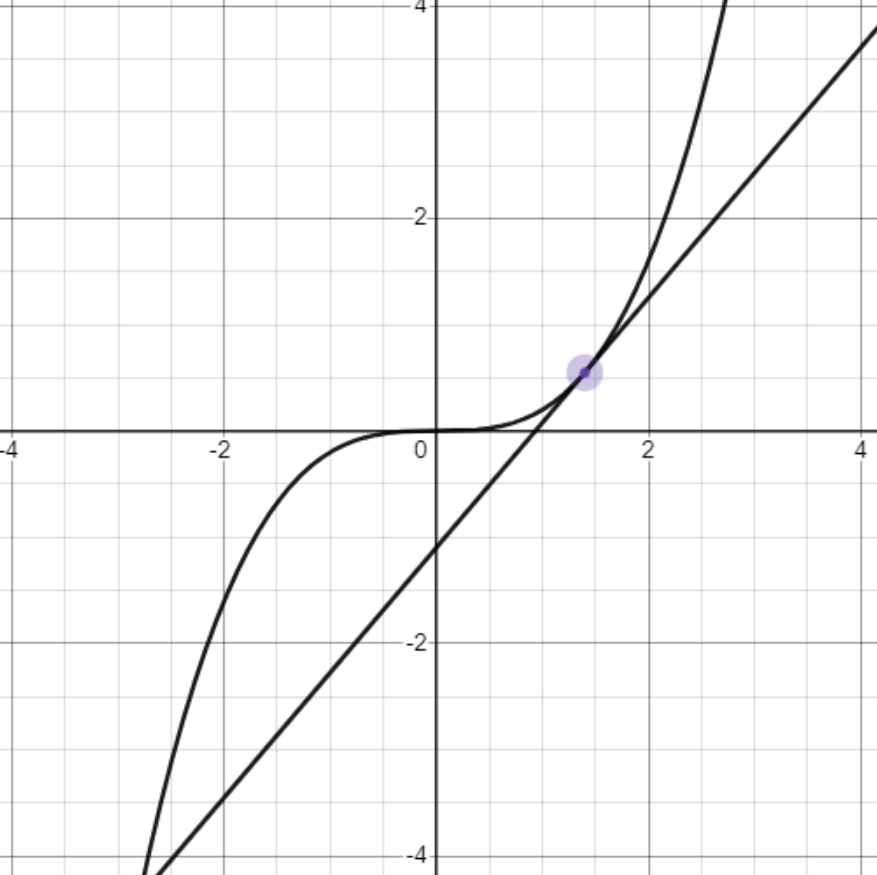
\includegraphics[height=2cm]{derivative.png} \hspace{2cm}  &  \textbf{Integral}   \hspace{2cm}  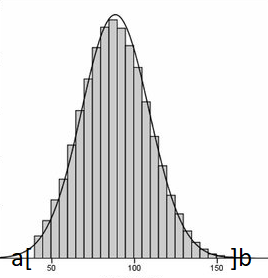
\includegraphics[height=2cm]{integral.png}  $\Delta x = \frac{b - a}{n}$ \\
$\frac{\Delta f(x)}{\Delta x} = \frac{f(x + \Delta x) - f(x)}{(x + \Delta x) - x}$  &  $\sum\limits_{i=a}^b f(x_i)\Delta x$ \\
$\lim_{\Delta x\to 0} \frac{f(x + \Delta x) - f(x)}{\Delta x} = \frac{df(x)}{dx}$  &  $\lim_{\Delta x\to 0}\sum\limits_{i=a}^b f(x_i)\Delta x = \int_{a}^b f(x)dx$ \\
\end{tabular}

\section*{The Fundamental Theorem of Calculus}
If a function \emph{f} is continuous on the closed interval [a, b] and \emph{F} is an anti-derivative of \emph{f} on the continuous interval [a, b], then $\int_{a}^b f(x)dx = F(b) - F(a)$

\subsection*{Approach - take the integral of a derivative of a function \emph{f(x)}}
Given that integration and differentiation are inverse operations taking the integral of the derivative should return the function itself f(x) in other words:  $\int \frac{df(x)}{dx}dx = f(x)$ \\
\emph{Intuition: } %?`$\sum\frac{\Delta f(x)}{\Delta x}\Delta x = \sum\frac{\Delta f(x)}{\cancel{\Delta x}}\cancel{\Delta x} = \sum\Delta f(x) = f(x)$ ? \\%
$\text{?`}\int \frac{df(x)}{\cancel{dx}}\cancel{dx} = \int df(x) = df(x)_1 + df(x)_2 + df(x)_3 + ... df(x)_n = f(x) + c$ ? \\

The fundamental theorem of calculus can be rewritten using in terms of \emph{F} as\\
$\int_{a}^b \frac{dF(x)}{dx}dx = F(b) - F(a)$ \hspace{1cm} | This can be proven as follows:\\
$\int_{a}^b \frac{dF(x)}{\cancel{dx}}\cancel{dx} = \int_{a}^b dF(x)$ \\%$ = \Eval{F(x)}{a}{b} = F(b) - F(a)$ \\
%$\sum\limits_{i=a}^b \frac{\Delta f(x_i)}{\Delta x}\Delta x = \sum\limits_{i=a}^b \Delta f(x_i)$ \\
Given $\Delta f(x) = f(x + \Delta x) - f(x) \hspace{0.5cm} \therefore \hspace{0.5cm} df(x) = f(x + dx) - f(x)$ \hspace{1cm} | The Integral can be written as an alternating series\\
$\int_{a}^b dF(x) = F(a + dx) - F(a) + F((a + dx) + dx) - F(a + dx) + F(((a + dx) + dx) + dx) - F((a + dx) + dx) + ... + F(a + ndx) - F(a + (n-1)dx)$ \hspace{1cm} 
| Every positive term can be canceled by subsequent negative term except for the negative term in the first sum and the positive term in the last sum\\
$\int_{a}^b dF(x) = \cancel{F(a + dx)} - F(a) + \cancel{F((a + dx) + dx)} - \cancel{F(a + dx)} + \cancel{F(((a + dx) + dx) + dx)} - \cancel{F((a + dx) + dx)} + ... + F(a + ndx) - \cancel{f(a + (n-1)dx)}$ \\
$\int_{a}^b dF(x) = F(a + ndx) - F(a)$ \hspace{1cm} | $b = a + n\Delta x \hspace{0.5cm}\therefore \hspace{0.5cm} a + ndx \rightarrow b$\\
$\int_{a}^b dF(x) = F(b) - F(a)$ \hspace{1cm} $\square$

\subsection*{Indefinite Integral}
$\int \frac{dF(x)}{dx}dx = \int \frac{dF(x)}{\cancel{dx}}\cancel{dx} = \int dF(x) = F(x) + C$ \hspace{1cm} | This can be proven as follows:\\
$\int dF(x) = \int_{x_0}^x dF(t)$ \hspace{1cm} | The indefinite integral can be rewritten using the change of variable technique as the definite integral $\int_{x_0}^x dF$ from an initial point $x_0$ to the variable x \\
Given $\Delta f(x) = f(x + \Delta x) - f(x) \hspace{0.5cm} \therefore \hspace{0.5cm} df(x) = f(x + dx) - f(x)$ 
\hspace{1cm} | The Integral can be written as an alternating series: $F(x_0 + dt) - F(x_0) + F((x_0 + dt) + dt) - F(x_0 + dt) + F(((x_0 + dt) + dt) + dt) - F((x_0 + dt) + dt) + ... + F(a + ndt) - f(a + (n-1)dt)$ 
\hspace{0.5cm} | The alternating terms cancel out except two terms \\
$\int_{x_0}^x dF(t) = \cancel{F(x_0 + dt)} - F(x_0) + \cancel{F((x_0 + dt) + dt)} - \cancel{F(x_0 + dt)} + \cancel{F(((x_0 + dt) + dt) + dt)} - \cancel{F((x_0 + dt) + dt)} + ... + F(a + ndt) - \cancel{f(a + (n-1)dt)}$  \\
$\int_{x_0}^x dF(t) = F(x_0 + ndx) - F(x_0)$ \hspace{1cm} | $x_0 + ndx \rightarrow x$\\
$\int_{x_0}^x dF(t) = F(x) - F(x_0)$ \hspace{1cm} | $x_0$ is a point $F(x_0) \rightarrow C$ \\
$\int dF(x) = F(x) + C$ \hspace{1cm} $\square$
\end{document}